\documentclass[a4paper]{article}

\usepackage{cmbright}
\usepackage[T1]{fontenc}

\usepackage{url}
\usepackage[all]{nowidow}

\usepackage[german]{babel}
\usepackage{csquotes}

\usepackage{fancyhdr}
\pagestyle{fancy}

\fancyhead{} % clear all header fields
\fancyhead[R]{Readme HybParc EKG-Einheit}
\fancyfoot{} % clear all footer fields
\fancyfoot[L]{\small{Readme version \today }}
\fancyfoot[R]{\thepage}

\usepackage{graphicx}
\graphicspath{ {./images/} }

\usepackage{xcolor}
\usepackage[colorlinks=true,colorlinks,
linkcolor=purple,
citecolor=purple,
urlcolor=blue,
filecolor=blue]{hyperref}
\usepackage[capitalise]{cleveref}

\newcommand{\warn}[1]{\textcolor{red}{#1}}
\newcommand{\code}[1]{\texttt{#1}}
\newcommand{\emoji}[1]{
    \begingroup\normalfont
    \includegraphics[height=0.8em]{emojis/#1.png}
    \endgroup
}

% for adjustwidth environment
\usepackage[strict]{changepage}

% for formal definitions
\usepackage{framed}

% environment derived from framed.sty: see leftbar environment definition
\definecolor{coolpurple}{rgb}{0.36,0.42,0.74}
\definecolor{formalshade}{rgb}{0.91,0.93,1}

\newenvironment{formal}{%
    \def\FrameCommand{%
    \hspace{1pt}%
    {\color{coolpurple}\vrule width 2pt}%
    {\color{formalshade}\vrule width 4pt}%
    \colorbox{formalshade}%
    }%
    \MakeFramed{\advance\hsize-\width\FrameRestore}%
    \noindent\hspace{-4.55pt}% disable indenting first paragraph
    \begin{adjustwidth}{}{7pt}%
    \vspace{2pt}\vspace{2pt}%
}
{%
    \vspace{2pt}\end{adjustwidth}\endMakeFramed%
}

\begin{document}

\begin{abstract}
    Dieses Readme deckt die Inbetriebnahme der am Medizinisches Interprofessionellen Trainingszentrum (MITZ) des Universitätsklinikum Dresden entwickelten EKG-Selbstlerneinheit für Studierende. Es beschreibt materielle und technische Voraussetzungen, ein empfohlenes räumliches Setup, Konfiguration und die Inbetriebnahme.
    Für substantielle Teile dieses Guides wird Unterstützung der Haus-IT benötigt, das Guide ist geschrieben für Ubuntu Linux.
\end{abstract}

\section{Materielle, Technische Voraussetzungen}
\label{sec:prerequisites}
Zur idealen Verwendung des Projektes wird benötigt
\begin{itemize}
    \item Eine medizinische Übungspuppe in Lebensgröße
    \item Ein EKG-Gerät mit 10 Elektroden + Klebepads
    \item Zwei USB-Kameras mit hoher Auflösung
    \item Ein PC zum Ausführen der Projektsoftware
    \item Ein Drucker, Klebeband und ein Klebestift
\end{itemize}

\subsection{USB-Kameras}
Für stabile Anwendung sind Kameras mit hoher Auflösung, 4K UHD oder höher, empfohlen. Das Originalsetup basiert auf zwei \enquote{HP 960 4K}. Das verwenden verschiedener Modelle ist meist möglich, solange die Kameras mit der gleichen Auflösung aufnehmen.


\subsection{PC}
\begin{formal}
    Dieser Teil sollte mit der IT-Abteilung besprochen werden.\emoji{technologist}\emoji{warning}
\end{formal}
Der PC benötigt mind. zwei freie USB-Ports (USB 2.0+). Das Projekt wurde mit Zielplattform Ubuntu Linux (\warn{Version abc-xyz}) entwickelt.

Auf dem PC muss die Umgebungsverwaltung Conda installiert sein. Aus Rechts- und Lizenzgründen sollte die über das Community-Projekt \href{https://conda-forge.org/}{Conda-Forge} bereitgestellte Variante (\enquote{miniconda}) genutzt werden. Das Projekt wurde mit Conda-Forge Version \warn{abc-xyz} entwickelt, sollte aber auch mit anderen Versionen funktionieren.

Nachdem conda installiert wurde, kann es im Terminal mit dem Befehl \code{conda} verwendet werden. Conda stellt isolierte Laufzeitumgebungen zur Verfügung und muss noch über das Terminal konfiguriert werden:
\begin{enumerate}
    \item Neue Umgebung erstellen: \code{conda create -n hybparc python=3.9}
    \item Neue Umgebung Aktivieren: \code{conda activate hybparc}
\end{enumerate}

Nun ist das offene Terminal auf die neue Umgebung gesetzt. Es müssen zuerst \enquote{Pip} (Python Paketmanager) und danach via Pip noch Python Pakete installiert werden. Sollte im Terminal nachgefragt werden, ob zusätzliche Abhängigkeiten (dependencies) mitinstalliert werden sollen, sollte dies mit \code{y} bestätigt werden.

\begin{enumerate}
    \item Pip installieren: \code{conda install pip}
    \item OpenCV installieren: \code{pip install opencv-contrib-python}
    \item PyQt6 installieren: \code{pip install pyqt6}
\end{enumerate}

Es sind alle dependencies des Projektes installiert, und das Projekt selbst kann heruntergeladen und konfiguriert werden.


\section{Projekinstallation, Konfiguration}
\begin{formal}
    Dieser Teil sollte mit der IT-Abteilung besprochen werden.\emoji{technologist}\emoji{warning}
\end{formal}
Es ist empfohlen, einen vorgefertigten Release von \warn{Twillo? Github?} herunterzuladen. Bei Bedarf steht der aktuelle Sourcecode auf \href{https://github.com/leloomi/hybparc_aruco}{GitHub} verfügbar.

Sollten die verwendeten Kameras die \textbf{exakt} gleiche Auflösung (3840x2160) wie die des Originalsetups haben, und MJPEG unterstützen, sollte das Projekt (unter Ubuntu Linux) nun ohne Probleme funktionieren. 

Potentiell müssen die interface IDs angepasst werden, diese können mit den v4l2 command line tools (müssen potentiell nachinstalliert werden) ausgelesen werden: \code{v4l2-ctl --list-devices}. Die Konfigurations-"Reihenfolge" der Kameras (Unterkörper vs. Oberkörper) spielt keine Rolle.

\subsection{Andere Auflösung 
\includegraphics[height=0.75em]{emojis/eyes.png}}
\label{sec:custom-resolution}
Bei anderen Auflösungen müssen im Code unter \code{/hybparc\_aruco/main.py} fast zu Beginn der \code{\_\_init\_\_} Funktion die entsprechenden Parameter angepasst werden:
\begin{figure}[h]
    \centering
    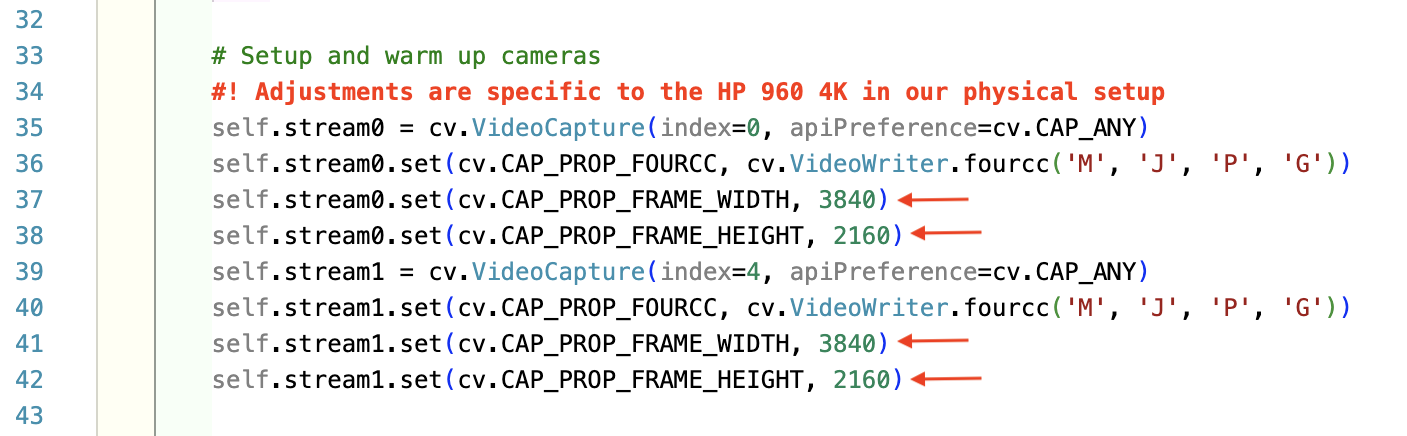
\includegraphics[width=10.5cm]{resolution.png}
\end{figure}

\subsection{Kein MJPEG 
\includegraphics[height=0.75em]{emojis/open-mouth.png}}
\label{ssec:the-mjpeg-problem}
Die unterstützten Formate einer Kamera bzw. Ihres Interfaces mit der Nr. X können via \code{v4l2-ctl -d /dev/videoX --list-formats-ext} ausgelesen werden. Der entsprechende Codec muss im \href{https://fourcc.org/codecs.php}{FourCC Format} unter \code{/hybparc\_aruco/main.py} fast zu Beginn der \code{\_\_init\_\_} Funktion angepasst werden:
\begin{figure}[h]
    \centering
    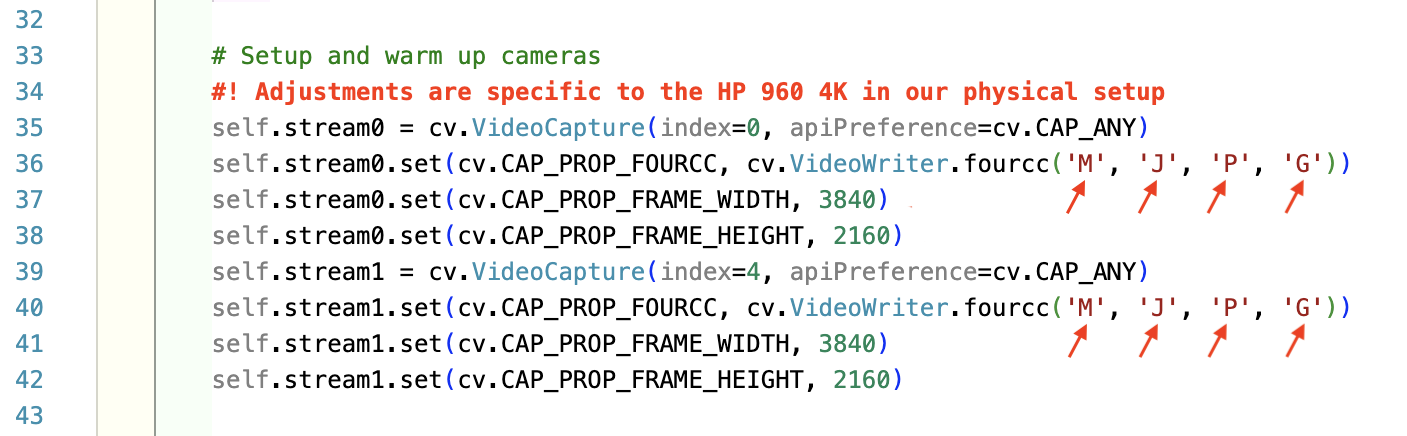
\includegraphics[width=10.5cm]{fourcc.png}
\end{figure}



\section{
\includegraphics[height=0.65em]{emojis/police-light.png} Troubleshooting 
\includegraphics[height=0.65em]{emojis/police-light.png}}
\label{sec:troubleshooting}

Um das Projekt über das Terminal zu starten, oder um Änderungen am conda environment vorzunehmen, muss das environment bei jedem Terminal neustart wieder aktiviert werden (\code{conda activate hybparc}).

\paragraph{OpenCV Package Type}
Das Guide empfiehlt \code{opencv-contrib-python} zu installieren. Dies ist eine Ubuntu Linux spezifische Empfehlung. Sollte das Projekt unter MacOS und Windows verwendet werden empfiehlt sich das Package \code{opencv-python}.

\end{document}